\documentclass{MIPRO}

\usepackage{cite}
\usepackage{amsmath,amssymb,amsfonts}
\usepackage{algorithmic}
\usepackage{graphicx}
\usepackage{textcomp}
\usepackage{xcolor}
\usepackage[T1]{fontenc}
\usepackage{flushend}
\usepackage{multirow}
\usepackage{multicol}
\usepackage{array}
\usepackage{url}
\usepackage{booktabs}
\usepackage{float}

\graphicspath{{../Picker-bot content/imgs/}}

\begin{document}

\title{Automated Component Recovery and Custom Kit Assembly System for Educational Circuit Kits}

\author{
\IEEEauthorblockN{
A. Mishra\IEEEauthorrefmark{1},
F. Mohammed\IEEEauthorrefmark{1},
J. Prasetyo\IEEEauthorrefmark{1}
}

\IEEEauthorblockA{\IEEEauthorrefmark{1}
Department of Computer Engineering and Informatics, Middlesex University Dubai, Dubai, UAE}

a.mishra@live.mdx.ac.uk, ff416@live.mdx.ac.uk, j.prasetyo@mdx.ac.ae
}

\maketitle

\begin{abstract}
Educational institutions frequently provide students with circuit development kits, such as Arduino modules, for practical coursework. However, when these kits are returned, they often lack critical components, rendering them unsuitable for redistribution as complete sets. This paper proposes an automated robotic solution to address this logistical and environmental inefficiency. Unlike traditional industrial assembly systems that merely construct standard products from uniform supply lines, the proposed system recovers components from existing, incomplete kits. Utilizing a machine vision system developed in Python, the system identifies available modules and communicates via TCP/IP with an EPSON RC8.0 simulator controlling a VT6-A901S 6-axis robot. This setup allows for the dynamic assembly of new kits based on custom Bills of Quantities (BOQs) submitted for specific projects. The result is a highly flexible, waste-reducing automated system that ensures students receive the exact components necessary for their modules.
\end{abstract}

\renewcommand\IEEEkeywordsname{Keywords}
\begin{IEEEkeywords}
\textit{Robotic Assembly, Machine Vision, Component Recovery, EPSON RC8.0, Automation, E-waste}
\end{IEEEkeywords}

\section{Introduction}

Practical electronics and robotics education heavily relies on the provision of development kits, predominantly featuring microcontrollers like the Arduino, alongside various sensors, actuators, and passive components. While students are generally encouraged to keep these kits for future innovation, some return them at the end of the academic term or leave their components in the form of assembled projects.

A significant problem arises during this return process: kits are frequently returned with missing, damaged, or misplaced modules. Because these returned kits are incomplete, they cannot be directly re-issued to incoming students who require standard, comprehensive module kits. Institutions thus face a build-up of partial kits, leading to unnecessary procurement costs and increased electronic waste.

To address this, an automated solution capable of processing these partial kits is needed. The objective of this project is to develop a robotic system that sorts through returned components and dynamically builds new kits. By focusing on project-specific requirements rather than rigid, standard kit definitions, the system ensures that even if a returned kit lacks certain generic parts, the components it does contain can be optimally reallocated to students based on their exact project needs.

\section{Methodology}

\subsection{Evaluation of Existing Solutions}

Automated kitting and assembly are well-established but they are almost exclusively designed for factory-stage production. Existing solutions primarily utilize Delta and SCARA (Selective Compliance Assembly Robot Arm) robots to pick and place uniform components from controlled feeder lines into packaging. Beyond factory stage production, automated sortation is also employed in large-scale waste management. For instance, facility-scale smart sortation systems utilize real-time machine vision combined with air jets and Delta robotic arms to autonomously recover valuable commodities, including e-waste, from mixed municipal solid waste streams~\cite{amp}. While these systems demonstrate the efficacy of AI-guided robotic sorting for high-volume material recovery, they operate on a facility scale designed for gross sorting rather than the precise, project-specific kitting of delicate microelectronic modules required in an educational setting.

These existing methodologies share a common limitation: they operate on the assumption of a continuous, uniform supply of new components. There is currently no widely adopted automated solution designed to recover loose, mixed components from pre-existing, partially depleted kits to create newly configured ones. Recent studies on automated e-waste recovery emphasize that the disassembly and salvaging of used electronics fundamentally differ from original production. Unlike new manufacturing, recovering used goods is characterized by high uncertainty, as components may be damaged, randomly oriented, or missing entirely~\cite{saenz}. Therefore, traditional deterministic factory automation is insufficient for these Re-X (Recycling, Re-use, Remanufacturing) activities, necessitating the flexible, data-driven robotic capabilities proposed in this project.

\subsection{Proposed Unique Approach}

The differentiating factor of the proposed solution lies in its intelligent recovery and flexible kitting approach. Rather than forcing staff to manually audit and sort thousands of individual components to rebuild standard kits, the system operates on a custom Bill of Quantities (BOQ) model.

Staff or students can submit custom project BOQs to the system. The automated system then identifies the required parts from the pool of returned components and selectively assembles a kit tailored specifically for that project. This transitions the institution from a ``push'' model (giving every student a standard kit regardless of need) to a ``pull'' model (assembling kits based strictly on project requirements), thereby maximizing the utility of returned inventory.

\section{Implementation}

To realize this automated recovery and assembly system, a simulated robotic workcell has been developed, integrating high-level software control with industrial robotic simulation.

\subsection{Machine Vision System}

\begin{figure}[t]
  \centering
  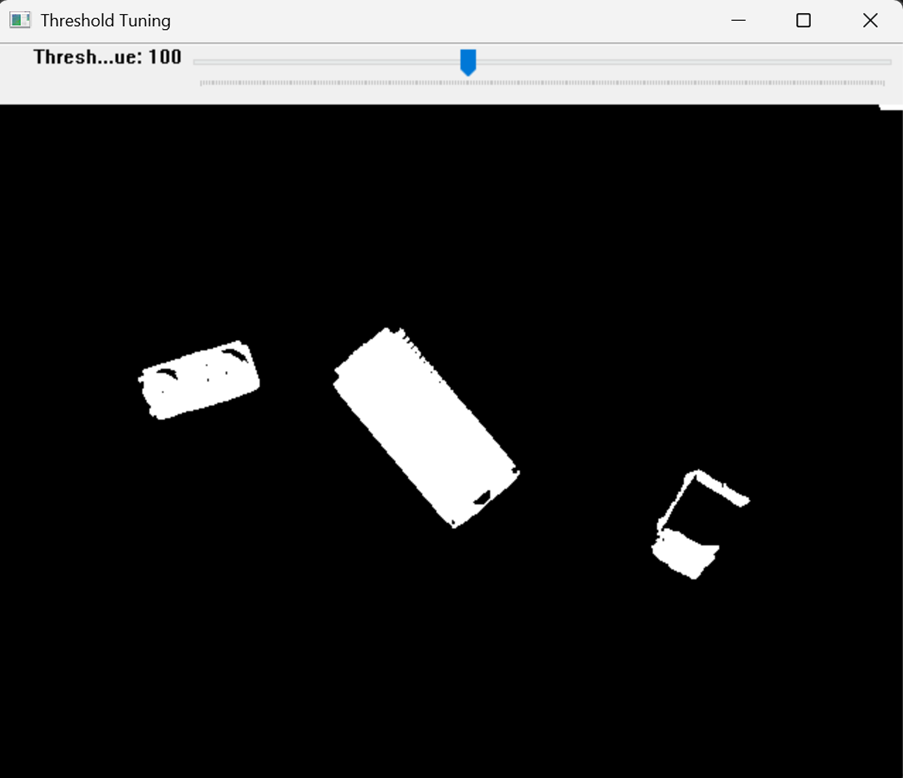
\includegraphics[width=\columnwidth]{threshold_pickerbot.png}
  \caption{Image thresholding using OpenCV during the prototype phase.}
  \label{fig:thresholding}
\end{figure}

The core intelligence of the automated pick-and-place operation lies within the machine vision architecture. This system is responsible for scanning the unstructured workbench domain, identifying electrical components, decoding their spatial orientation, and translating native pixel data into rigid Cartesian kinematics for the EPSON VT6-A901S manipulator. While many advanced industrial bin-picking solutions rely on line-of-sight 3D cameras, these sensors generate point clouds that are highly susceptible to spurious outliers when scanning cluttered, overlapping parts. These outliers can spoil a robot's obstacle avoidance planning and impede component segmentation, thus requiring computationally demanding filtering procedures~\cite{Franaszek}. To bypass the complexities of 3D point cloud filtration and maintain efficient real-time processing, this project deliberately utilizes a 2D planar overhead vision approach. The development of this system progressed through two distinct phases, ultimately culminating in an industrial-grade deep learning solution.

\subsubsection{Prototype Phase: Deterministic Computer Vision}

The initial pipeline applied Gaussian blurring and global binary thresholding (Fig.~\ref{fig:thresholding}) to isolate component footprints, then used \texttt{cv2.findContours} to extract boundaries. Sub-images were padded to 224$\times$224 tensors and classified with a Google Teachable Machine model. While functional in controlled conditions, the prototype collapsed under minor environmental changes: metallic glare erased texture data, background clutter produced false ``Noise'' classifications, and axis-aligned bounding boxes were incapable of recovering component rotation angle.

\subsubsection{Final Architecture: YOLOv8-OBB}

\begin{figure}[t]
  \centering
  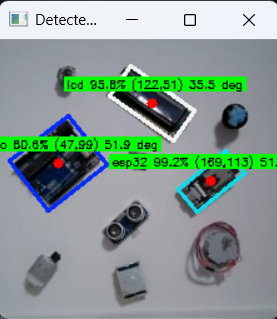
\includegraphics[width=\columnwidth]{yolo_detect_v2.png}
  \caption{Real-time component detection with YOLOv8-OBB, showing oriented bounding boxes and per-class confidence scores.}
  \label{fig:yolo-detect}
\end{figure}

To resolve the catastrophic limitations of standard classification, the system was entirely re-architected around a YOLOv8-OBB state-of-the-art neural network. Rather than attempting to manually threshold and isolate items via algorithmic cropping, the YOLOv8 engine ingests the full-resolution uncropped camera frame in real time. Hyper-trained on a custom, heavily augmented Computer Vision Annotation Tool (CVAT) dataset featuring extreme lighting shifts and rotational variances, the OBB model dynamically bypasses all glare and localized clutter (Fig.~\ref{fig:yolo-detect}). While the manual image annotation required for this supervised learning approach demands significant engineering preparation time, recent comparative studies in robotic kitting demonstrate it is a necessary trade-off to achieve the high recognition quality and precise spatial accuracy required for successful bin-picking~\cite{Fager}. In a single forward pass, the deep convolutional layers output a 5-dimensional oriented tensor $\langle cx, cy, w, h, \theta \rangle$ alongside deterministic multi-class probabilities (Arduino, ESP32, LCD). This streamlines the recovery process compared to other recent robotic bin-picking solutions which rely on multi-stage hybrid pipelines---such as using YOLOv5 for initial top-view detection followed by an eye-in-hand camera movement to perform FAST and BRISK feature-matching for pose estimation~\cite{Taweesoontorn}. By natively deriving the resting rotation angle $\theta$ from a single overhead frame, the proposed OBB architecture entirely decoupled the system's reliance on perfect environmental lighting and complex multi-step image capture.

\subsubsection{Logistics Filtering and BOQ Engine}

Once the vision system successfully extracts the precise $x$ and $y$ pixel centroids alongside the target item's class label, an intelligent logistics filter operates actively above the vision loop frame buffer. Rather than greedily passing every single detected piece of hardware down into the spatial coordinate mapping pipeline, the vision orchestrator interfaces natively with the BOQ model. The system evaluates the raw visual output and intelligently matches the detected inventory against the required logistical payload. It safely filters out and ignores surplus components even if they geometrically validate, ensuring that only precisely kitted workloads are forwarded to the spatial calibration engine for EPSON translation.

\subsection{Spatial Calibration and Coordinate Mapping}

\begin{figure}[t]
  \centering
  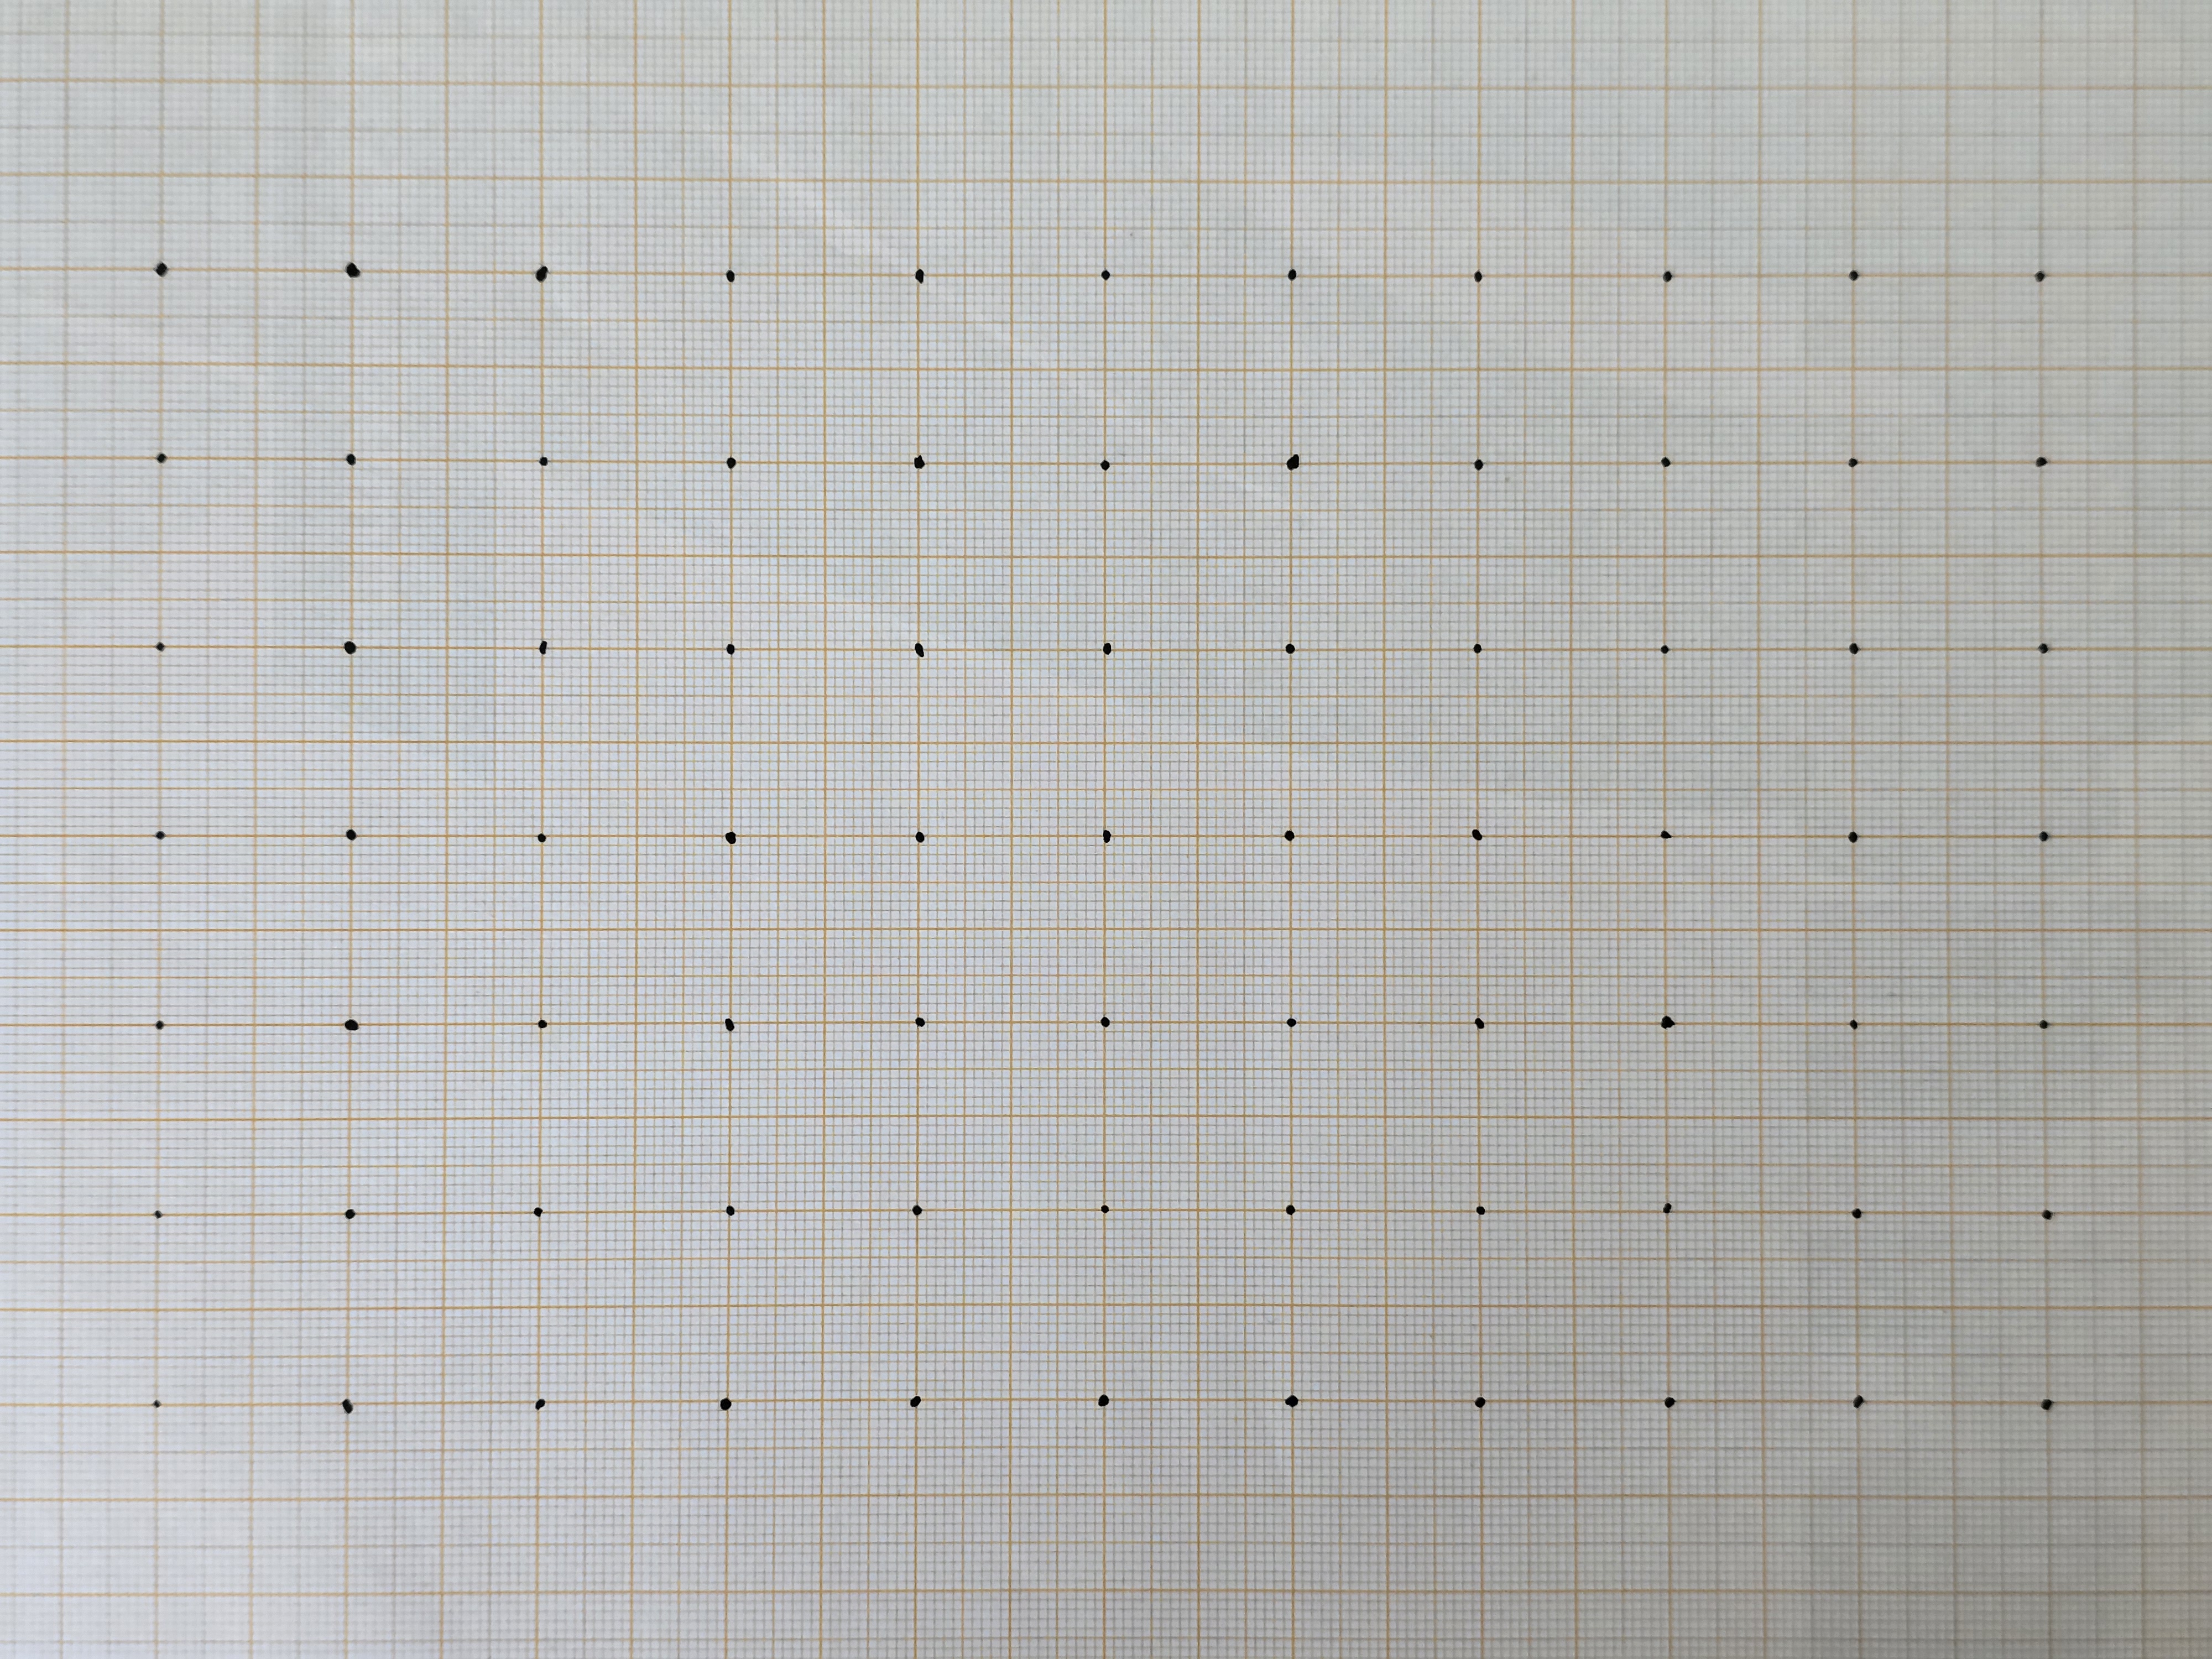
\includegraphics[width=\columnwidth]{graph_paper.jpg}
  \caption{77-point homography calibration grid (11$\times$7 at 20\,mm spacing) overlaid on the workspace reference image.}
  \label{fig:calibration_grid}
\end{figure}

A critical requirement of the system is the ability to translate pixel positions in the camera image into physical millimetre coordinates within the robot's world frame. This is achieved through a planar homography transformation, which provides a projective mapping between the two coordinate spaces.

To establish this mapping, a 77-point calibration grid is used, arranged as 11 columns and 7 rows on the workspace surface with 20\,mm spacing (Fig.~\ref{fig:calibration_grid}). The world $X$-coordinate of each column decreases from $+100$\,mm to $-100$\,mm left to right, and the world $Y$-coordinate increases from 410\,mm to 530\,mm top to bottom, yielding a calibrated area of $200\,\text{mm} \times 120\,\text{mm}$. A reference image of the grid is captured and \texttt{tools/calibration\_clicker.py} is used to click each of the 77 intersection points. A second utility, \texttt{tools/sort\_and\_tag\_pixels.py}, sorts the recorded pixel coordinates and appends the corresponding world coordinates to produce a four-column CSV file.

The homography matrix $\mathbf{H}$ is computed using OpenCV's \texttt{findHomography} with the standard least-squares (SLS) method rather than RANSAC. This choice is deliberate: the RANSAC estimator is designed to reject outliers, but the corner calibration points represent valid boundary constraints. Treating them as potential outliers would introduce systematic error near the workspace boundaries. At runtime, any detected pixel centroid $(p_x, p_y)$ is transformed to world coordinates $(w_x, w_y)$ via \texttt{cv2.perspectiveTransform} with $\mathbf{H}$.

When the camera is repositioned vertically, the physical scale of the image changes, invalidating the original pixel-to-millimetre mapping. A height recalibration routine invoked via \texttt{pickerbot.py -{}-calibrate} addresses this without requiring a full recalibration. A reference image is presented to manually select two points 20\,mm apart on a ruler image; the pixel distance between those clicks is measured and a scale factor is computed. Let $r_h$ and $r_v$ denote the mean pixel distance per 20\,mm in the horizontal and vertical axes from the original calibration. For a ruler measurement at angle $\theta$ relative to the horizontal, the expected pixel distance is:

\begin{equation}
  d_{\mathrm{expected}} = \sqrt{\left(r_h \cos\theta\right)^2 + \left(r_v \sin\theta\right)^2}
  \label{eq:expected_dist}
\end{equation}

where $\theta = \arctan2(|\Delta y|, |\Delta x|)$. The scale factor is then:

\begin{equation}
  s = \frac{d_{\mathrm{measured}}}{d_{\mathrm{expected}}}
  \label{eq:scale_factor}
\end{equation}

This formulation accounts for the fact that horizontal and vertical pixel densities may differ due to lens geometry or non-square pixel sampling. All 77 pixel coordinates are scaled around the grid centre point (index 38) by $s$, and the adjusted calibration is written to \texttt{calibration\_pixels\_scaled.csv} and referenced in \texttt{config.json} for all subsequent runs.

\subsection{TCP/IP Communication Protocol}

\begin{table}[t]
  \caption{TCP/IP Command Set}
  \label{tab:commands}
  \renewcommand{\arraystretch}{1.35}
  \centering
  \setlength{\tabcolsep}{4pt}
  \begin{tabular}{@{} l l p{3.3cm} c @{}}
    \toprule
    \textbf{Command} & \textbf{Params} & \textbf{Robot Action} & \textbf{Reply} \\
    \midrule
    \texttt{JUMP}    & x, y, z, u & Lift 50\,mm, translate to $(x,y,z{+}50)$, descend to $(x,y,z,u)$ & \texttt{OK} \\[2pt]
    \texttt{GO}      & x, y, z    & Linear move to $(x,y,z)$                                         & \texttt{OK} \\[2pt]
    \texttt{MOVE}    & x, y, z    & Linear move to $(x,y,z)$                                         & \texttt{OK} \\[2pt]
    \texttt{PICK}    & x, y, z, u & Full pick-and-place sequence (Sec.~\ref{sec:epson})               & \texttt{OK} \\[2pt]
    \texttt{STANDBY} & ---        & Return to home position                                           & \texttt{OK} \\
    \bottomrule
  \end{tabular}
\end{table}

The Python control system communicates with the EPSON RC8 controller over a local TCP socket connection. For simulation the target address is \texttt{127.0.0.1} on port 2001; when connecting to the physical robot the address is changed to \texttt{192.168.X.Y} via \texttt{config.json}. All connection management and command dispatch is handled by the \texttt{pickerbot\_lib.sender} module, which maintains a module-level socket object across the lifecycle of a session.

Commands are transmitted as plain ASCII strings in the format \texttt{CMD~X~Y~Z~U\textbackslash r\textbackslash n}, where $X$, $Y$, $Z$ are world coordinates in millimetres and $U$ is the tool rotation angle in degrees. The controller must reply \texttt{OK} before the next command is issued (Table~\ref{tab:commands}). In multi-component batch pick operations, the \texttt{epsonPickAll} function iterates over a list of world-coordinate strings, issuing a \texttt{PICK} command for each. Any non-\texttt{OK} response immediately aborts the batch and returns the arm to standby, ensuring that a partial failure such as a grip error or controller fault does not result in further motion in an undefined mechanical state.

\subsection{EPSON RC8 Robot Program}
\label{sec:epson}

\begin{figure}[t]
  \centering
  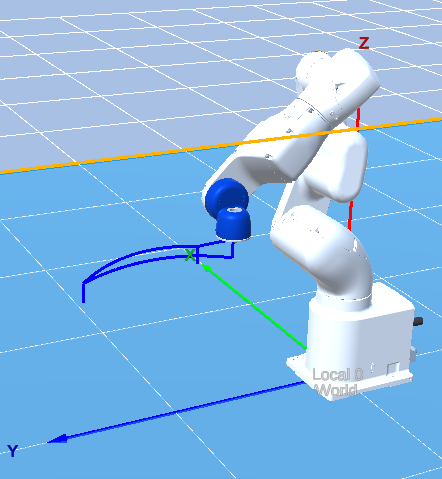
\includegraphics[width=\columnwidth]{pick_trajectory.png}
  \caption{Trajectory of the \texttt{PICK} command: three-phase Jump3 approach, gripper activation, transport to \texttt{PlacePoint}, and retract to standby.}
  \label{fig:pick_trajectory}
\end{figure}

The robot-side program (\texttt{Epson/Pickerbot\_Receiver/Main.prg}) is written in Epson SPEL+, the proprietary scripting language for the RC8 controller, using a community TCP template~\cite{prasetyo2024} with predefined motion initialization parameters. After initialization it opens a TCP server on network channel \#201 at port 2001 and waits for an incoming client connection before entering its command-processing loop.

Each received string is parsed by space delimiter, with the first token identifying the command and subsequent tokens providing coordinate arguments as floating-point values. The \texttt{PICK} command implements the most complex motion sequence (Fig.~\ref{fig:pick_trajectory}): the arm first lifts vertically from its current position, then translates horizontally to an elevated waypoint at $(x, y)$ with tool orientation $u$, and finally descends to the exact pick position. Once there, a digital output closes the gripper and a dwell time ensures a reliable mechanical grip. The robot then executes a second Jump3 sequence, lifting clear of the workspace and traveling to the predefined \texttt{PlacePoint} container, before deactivating the gripper output and returning to standby. A network error handler attempts to reopen the server socket on transient faults, allowing the system to recover without human intervention.

\subsection{Software Architecture and Entry Points}

\begin{figure}[t]
  \centering
  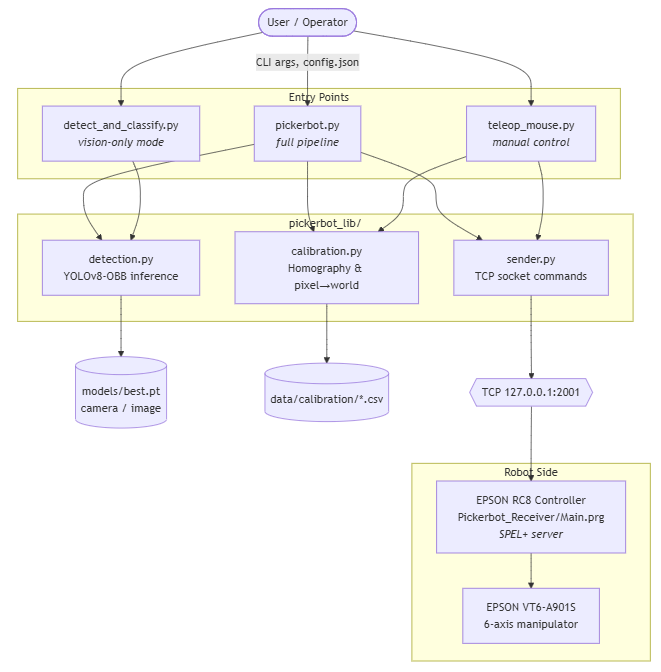
\includegraphics[width=\columnwidth]{software_architecture.png}
  \caption{Picker-Bot software architecture: three entry-point scripts sharing the \texttt{pickerbot\_lib} package containing \texttt{detection}, \texttt{calibration}, and \texttt{sender} submodules.}
  \label{fig:architecture}
\end{figure}

The Python codebase is structured around the \texttt{pickerbot\_lib} shared library package, consolidating detection, calibration, and TCP communication into three importable submodules: \texttt{detection}, \texttt{calibration}, and \texttt{sender} (Fig.~\ref{fig:architecture}). Three entry-point scripts serve distinct operational modes. \texttt{pickerbot.py} orchestrates end-to-end pick sessions, loading calibration, running detection, and dispatching pick commands over TCP. \texttt{detect\_and\_classify.py} isolates the vision layer for development, exposing a live confidence threshold slider without a robot connection. \texttt{teleop\_mouse.py} enables manual arm positioning by transforming mouse clicks on the calibration image through the homography matrix and issuing \texttt{MOVE} commands, allowing spatial accuracy to be verified before automated operation.

\subsection{Robotic Control and Simulation}

The physical manipulation of components is simulated using the EPSON RC8.0 software environment. For the initial setup, a physical evaluation space of $200\,\text{mm} \times 120\,\text{mm}$ and a deposit spot 280\,mm above the workspace centre were used to create the mapping. The chosen robotic platform is the EPSON VT6-A901S~\cite{b2}, a 6-axis articulated robot arm with 980\,mm reach providing the approach-angle flexibility and high repeatability required for precise pick-and-place operations. Detailed installation, safety, and operational specifications are outlined in the official Epson VT6 series documentation~\cite{epsonvt6}.

\section{Results}

The implementation of the Picker-Bot system achieved a cohesive integration of deep-learning-based computer vision with industrial robotic control inside the EPSON RC8.0 simulation environment. The following subsections describe the observed behaviour of the system across its three principal layers of responsibility: perception, spatial reasoning, and supervised manipulation.

\subsection{Vision System Performance and Robustness}

\begin{figure}[t]
  \centering
  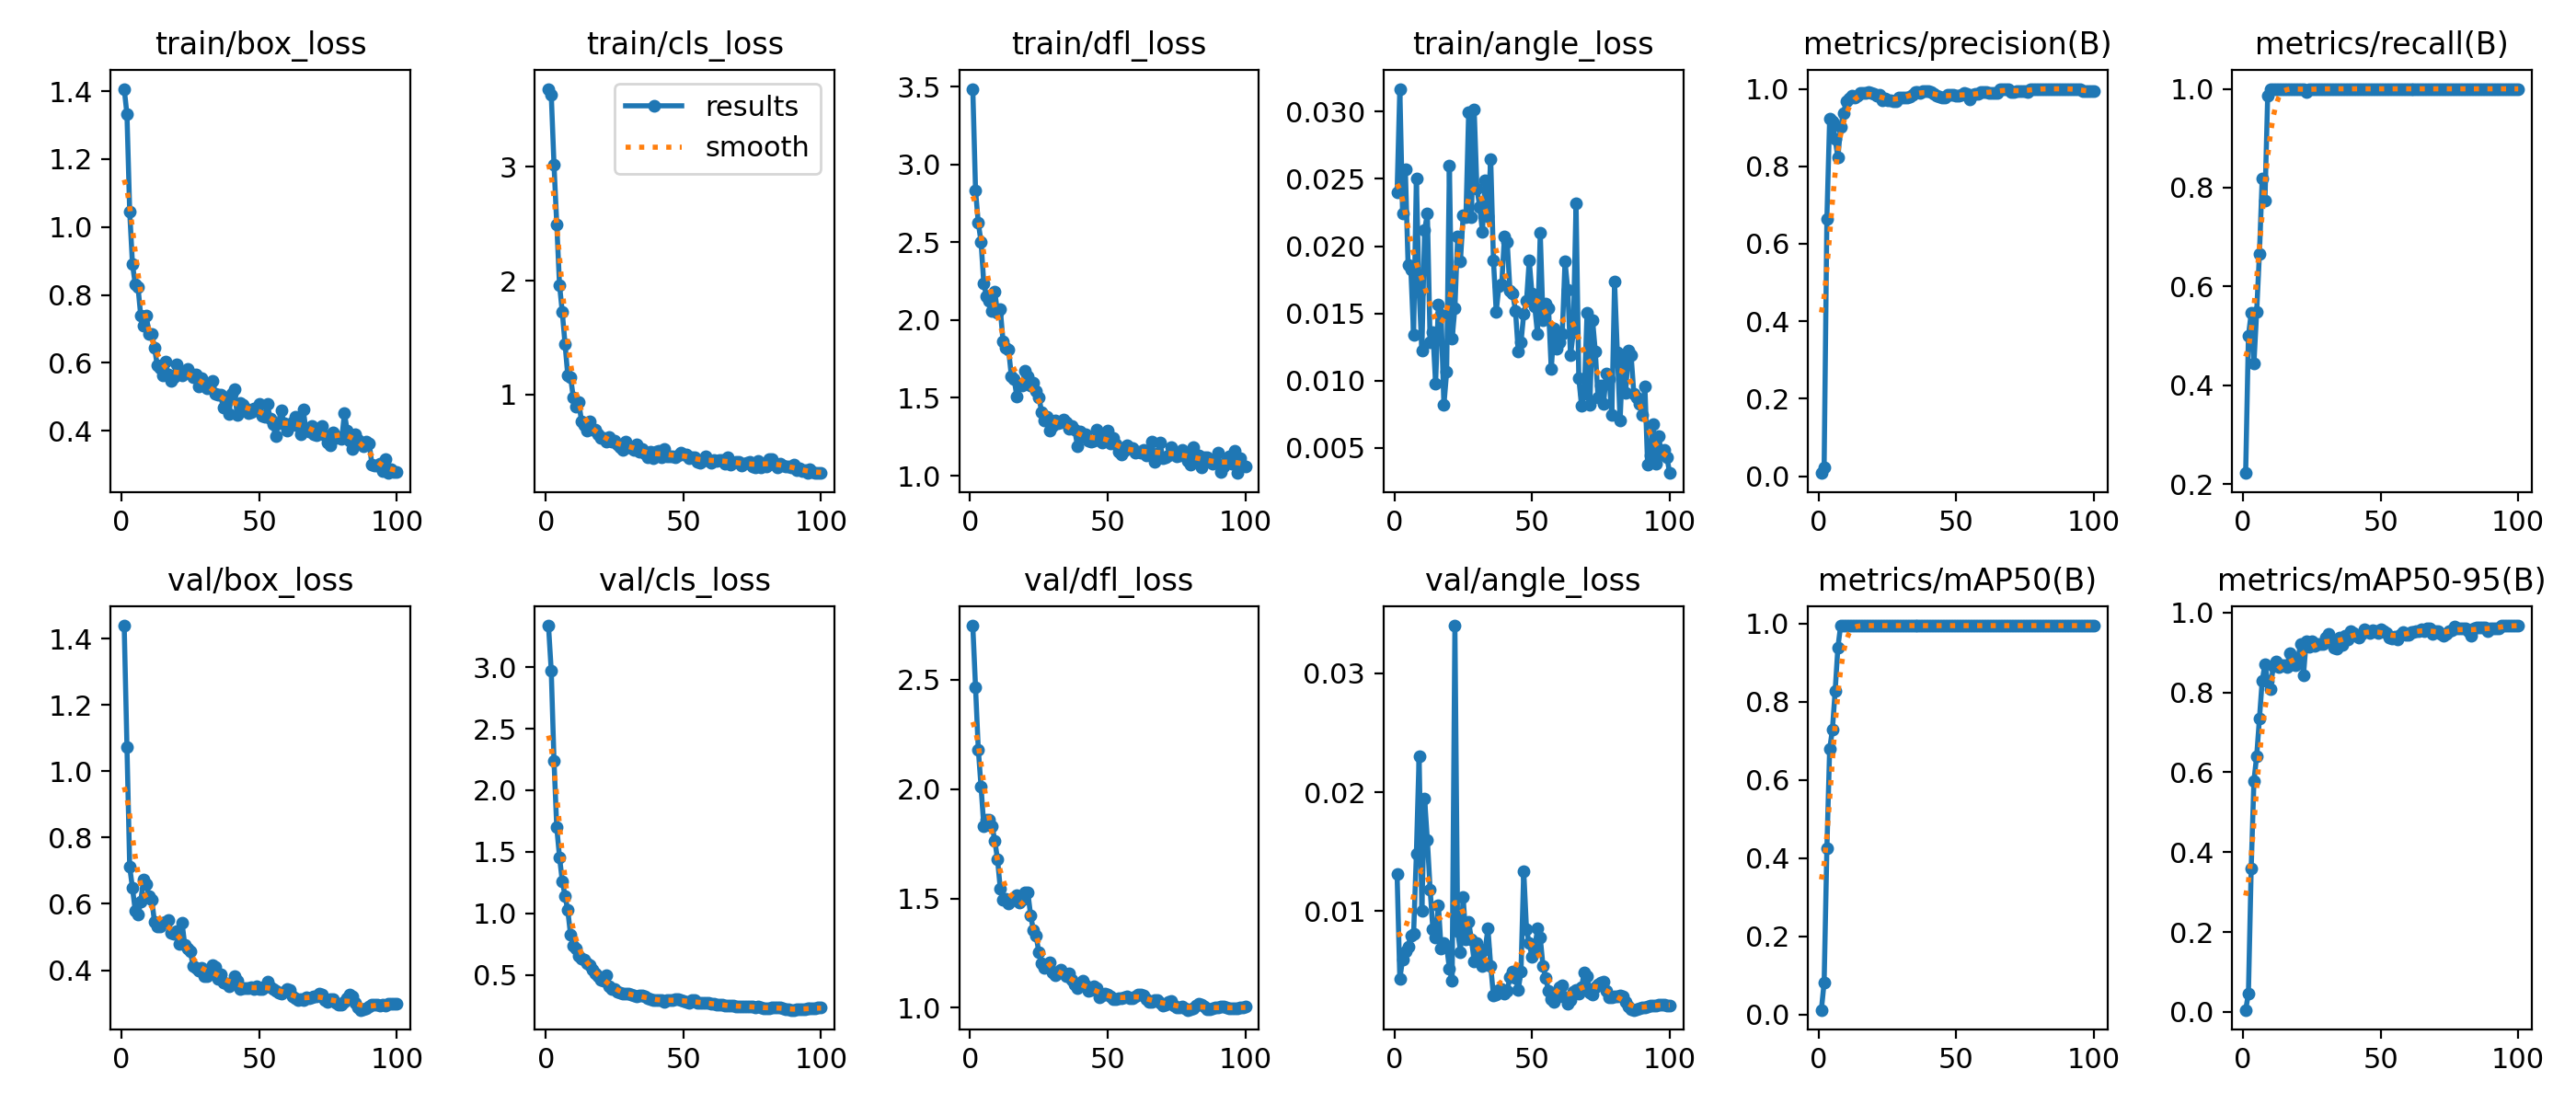
\includegraphics[width=\columnwidth]{yolo_results.png}
  \caption{YOLOv8-OBB training metrics: loss curves and $mAP_{50}$ progression demonstrating rapid convergence and high detection accuracy on the in-distribution component set.}
  \label{fig:yolo_results}
\end{figure}

The migration from a deterministic OpenCV prototype to the YOLOv8-OBB architecture produced a substantial improvement in detection reliability. The final model identified and classified Arduino, ESP32, and LCD modules within a single forward pass, recovering the resting rotation angle $\theta$ alongside the pixel centroid $(cx, cy)$ for each detected component without any auxiliary geometric post-processing. The learned representation absorbed much of the environmental variability that had previously destabilised the pipeline, including metallic glare from populated boards, localised clutter around the workpiece, and residual background texture. An explicitly trained ``noise'' class was suppressed at the output stage, ensuring only valid components were forwarded to the coordinate mapping layer.

The quantitative evaluation is summarised in Fig.~\ref{fig:yolo_results}, which plots the loss curves and mean Average Precision over the course of training. The model converged rapidly and reached a final $mAP_{50}$ of 0.99, indicating near-perfect localisation and classification within the training distribution. A fixed confidence threshold of 0.7 eliminated the small number of remaining false positives attributable to glare artefacts, without requiring additional non-maximum suppression or hand-tuned filtering downstream.

\subsection{Spatial Calibration and Mapping Accuracy}

The homography-based calibration provided a reliable bridge between the two-dimensional camera image and the planar subset of the robot's workspace. The 77-point reference grid defined a calibrated operating region of approximately $200\,\text{mm} \times 120\,\text{mm}$ and covered the full region of interest visible to the overhead camera. The use of a standard least-squares solution for \texttt{findHomography}, rather than a RANSAC-based estimator, was an intentional design choice: it ensured that corner points on the workspace boundary were not discarded as statistical outliers, which would otherwise have contracted the effective calibrated area.

The height recalibration routine handled the practical problem of camera repositioning without requiring the user to re-click every grid intersection. By measuring a known 20\,mm ruler segment in the new image and comparing its pixel length against the expected distance implied by the original horizontal and vertical grid pitches, the routine recovered an anisotropic scale factor and applied it uniformly around the grid centre. In testing this allowed vertical camera adjustments to be absorbed in seconds, with the resulting transformation verified interactively through \texttt{teleop\_mouse.py}: each click on the calibration reference image translated into a physical \texttt{MOVE} command whose terminal position agreed visually with the clicked feature.

\subsection{Integrated Robot Control and Logistics}

The combined control pipeline exercised the intended pull-based kitting behaviour end-to-end. When a BOQ was supplied, the system satisfied requirements in order of detection confidence and silently ignored surplus components---the behaviour expected of a logistics auditor rather than a greedy collector. In the absence of a BOQ it reverted to greedy mode and picked every non-noise detection. The full TCP command vocabulary was validated across extended simulation runs, with each command confirmed by \texttt{OK} before the next was dispatched. Synthetic fault injection verified that the abort-on-failure strategy correctly returned the arm to standby rather than advancing through an undefined mechanical state.

\section{Future Discussion}

While the current implementation successfully demonstrates the concept within a simulated environment, several avenues remain open. The most immediate step is transitioning to a physical VT6-A901S unit, requiring camera calibration under real lighting conditions, per-component gripper timing, and potentially a compliant gripper for delicate modules. Looking further ahead, a web portal for BOQ submission would make the system self-service, while IoT-guided AGVs~\cite{vlachos} could automate bin transport between storage and the workcell, completing the pull-model logistics pipeline end-to-end.

\section{Conclusion and Discussion}

\subsection{Critical Evaluation of System Integration}

The development of the Picker-Bot system successfully transitioned from a standard industrial ``push'' model to a project-specific ``pull'' model for component kitting. The technical cornerstone of this project was the migration from deterministic OpenCV prototypes to the YOLOv8-OBB architecture. While the initial prototype was highly sensitive to environmental shifts, the final deep-learning model achieved a $mAP_{50}$ of 0.99, proving that high-accuracy bin-picking is viable in cluttered educational environments without the hardware overhead of 3D point-cloud sensors. The system's ``logistics auditor'' approach---using the BOQ engine to filter detections---ensures that the vision system both sees parts and intelligently manages inventory. By ignoring surplus components and focusing only on project requirements, the system directly addresses the original goal of reducing procurement costs and e-waste.

\subsection{Implementation Constraints and Real-World Considerations}

While the simulation in EPSON RC8.0 was successful, the present implementation carries a number of constraints that any physical deployment would need to address. The software-enforced inter-command delay was instrumental in keeping the simulated motion pipeline stable, but a fixed guard of this kind is unlikely to survive contact with real hardware unchanged. A physical workcell would benefit from a delay tuned to the inertial characteristics of the component currently being handled, since a heavier module such as the LCD settles differently from a lighter one such as the ESP32.

The 77-point homography establishes a robust two-dimensional correspondence across the work surface, but remains a planar model of what is in practice a three-dimensional problem. Components of non-negligible height introduce a parallax offset that a purely planar calibration cannot account for, and which would manifest during the descending phase of the Jump3 trajectory as a small but systematic lateral error. Future directions would therefore need to incorporate a height-aware correction, either through explicit per-class offsets or through the introduction of a depth sensor.

\subsection{Concluding Remarks}

In conclusion, the Picker-Bot system provides a technically sound and environmentally sustainable solution for managing returned educational circuit kits. By integrating Oriented Bounding Box detection, planar homography, and TCP/IP-based control, the project demonstrates that modern AI can transform ``loose waste'' into valuable, project-ready assets. This implementation sets a precedent for how robotics can be applied to Re-X (Recovery and Re-use) activities within specialised microelectronic environments, effectively bridging the gap between waste management and logistical efficiency.

\section*{acknowledgment}

The authors acknowledge the guidance and resources provided throughout the PDE4435 module at Middlesex University Dubai, which encouraged a design-thinking approach to advanced robotics projects. They also acknowledge the use of Claude AI during project development.

\begin{thebibliography}{00}
\bibitem{amp}
AMP, ``AMP ONE: Automated Waste Sorting Systems \& Facility,'' 2026. [Online]. Available: \url{https://ampsortation.com/products/amp-one}.

\bibitem{saenz}
J.~Saenz \textit{et al.}, ``Automated disassembly of e-waste---requirements on modeling of processes and product states,'' \textit{Frontiers in Robotics and AI}, vol.~11, p.~1303279, 2024.

\bibitem{Franaszek}
M.~Franaszek, P.~Rachakonda, and K.~S.~Saidi, ``Filtering Organized 3D Point Clouds for Bin Picking Applications,'' \textit{Applied Sciences}, vol.~14, no.~3, p.~961, Jan.~2024.

\bibitem{Fager}
P.~Fager, R.~Hanson, \AA.~Fasth-Berglund, and S.~Ekered, ``Supervised and unsupervised learning in vision-guided robotic bin picking applications for mixed-model assembly,'' \textit{Procedia CIRP}, vol.~104, pp.~1304--1309, 2021.

\bibitem{Taweesoontorn}
T.~Taweesoontorn, S.~Yanyong, and P.~Konghuayrob, ``Hybrid Deep Learning and FAST--BRISK 3D Object Detection Technique for Bin-picking Application,'' \textit{Sensors and Materials}, vol.~36, no.~4, pp.~1389--1404, 2024.

\bibitem{prasetyo2024}
J.~Prasetyo, ``RC7\_Python,'' Jan.~2024. [Online]. Available: \url{https://github.com/judhi/RC7_Python}.

\bibitem{b2}
EPSON Robotics, ``RC8.0 Reference Manual,'' EPSON Factory Automation, 2023. [Online]. Available: \url{https://www.epson.com}.

\bibitem{epsonvt6}
Epson America, Inc., ``Epson VT6L All-in-One 6-Axis Robots,'' Epson US, 2026. [Online]. Available: \url{https://epson.com/Support/Robots/6-Axis-Robots/VT-Series/Epson-VT6L-All-in-One-6-Axis-Robots/s/SPT_VT6L-A901SS}.

\bibitem{vlachos}
I.~Vlachos \textit{et al.}, ``Smart and flexible manufacturing systems using Autonomous Guided Vehicles (AGVs) and the Internet of Things (IoT),'' \textit{Int. J. Production Research}, pp.~1--22, 2022.
\end{thebibliography}

\end{document}
